\documentclass{beamer}

\usepackage[utf8]{inputenc}
\usepackage[ngerman]{babel}

\mode<presentation> {
  %\setbeameroption{show notes} % Kommentare im fertigen PDF

  \usetheme{Boadilla}
  \usecolortheme{seagull}

  \setbeamertemplate{footline}[page number] % Einfacher Folienzähler als Fußzeile
  \setbeamertemplate{navigation symbols}{} % Keine Navigationslinks
}

\usepackage{graphicx} % Zum Bilder-Einbinden
\usepackage{mdframed} % Farbige Boxen

% Damit die Tilde ~ im Code nicht hochgestellt dargestellt wird, muss man einen anderen Font verwenden, z.B.
%\usepackage[T1]{fontenc}
%\usepackage{beramono}
% Dieser Font ist aber zu breit.
% siehe https://github.com/gpoore/minted/issues/2#issuecomment-18451836
\usepackage[outputdir=output]{minted} % Syntax-Highlighted Code; requires pygments to be installed
\newminted{haskell}{}
\newmintinline{haskell}{}

\usepackage{hyperref}
\usepackage{url}
% URLs mit LaTeX-Sonderzeichen (Prozent-Zeichen etc.)
\urldef{\lenswithoutdep}\url{https://github.com/ekmett/lens/wiki/How-can-I-write-lenses-without-depending-on-lens%3F}

\usepackage{tikz}
\newcommand\marktikz[1]{%
  \tikz[remember picture,overlay] \node[inner xsep=0pt] (#1) {};
}
\tikzstyle{typeline}=[yellow, very thick]
\tikzstyle{typebox}=[black, fill=yellow, align=left]
\tikzset{onslide/.code args={<#1>#2}{%
  \only<#1>{\pgfkeysalso{#2}} % \pgfkeysalso doesn't change the path
}}

\definecolor{dimgray}{rgb}{0.41, 0.41, 0.41}
\definecolor{greenncs}{rgb}{0.0, 0.62, 0.42}

\usepackage{colortbl} % Farbige Gitter in Tabellen

% Bildquelle: http://www.dibujosdisneyparacolorear.com/imagenes-donald-detective-jpg
\setbeamertemplate{background}{
\includegraphics[width=\paperwidth,height=\paperheight,keepaspectratio]{images/donald-detective-bg.jpg}}

\defbeamertemplate*{title page}{customized}[1][]
{
  \centering
  \usebeamerfont{title}{\LARGE \inserttitle}\par
  \usebeamerfont{subtitle}\usebeamercolor[fg]{subtitle}\insertsubtitle\par
  \bigskip
  \usebeamercolor[fg]{titlegraphic}\inserttitlegraphic\par
  \bigskip
  \usebeamerfont{author}\insertauthor\\[0.5em]
  \usebeamerfont{institute}\insertinstitute\par
  \usebeamerfont{date}\insertdate\par
}

\title[Lens]{Lenses und Zauberwürfel}
\titlegraphic{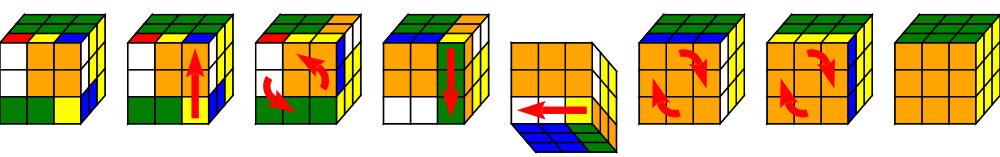
\includegraphics[width=0.65\linewidth]{images/rubiks-sequence.png}}
\author{Tim Baumann}
\institute[CCA]{Curry Club Augsburg}
\date{13. August 2015}

\newcommand{\kreuz}{$\,^\dag$} % Dagger, alter!
\newcommand{\kkreuz}{$\,^\ddag$} % DDagger, alter!
\newcommand{\fa}{$\forall$}
\newcommand{\ev}{$\rightsquigarrow$} % evaluates to
\newcommand{\hl}[1]{\colorbox{yellow}{#1}} % highlight code
\newcommand{\hll}[1]{\colorbox{yellow!50!white}{#1}} % highlight code (weaker)

\begin{document}

\begin{frame}
  \titlepage
\end{frame}

\iffalse
\begin{frame}
  \frametitle{Übersicht}
  \tableofcontents
\end{frame}
\fi

\begin{frame}[fragile,t]
  \frametitle{Welche Bibliothek?}
  % Bildquelle: https://ro-che.info/ccc/23
  \begin{figure}
    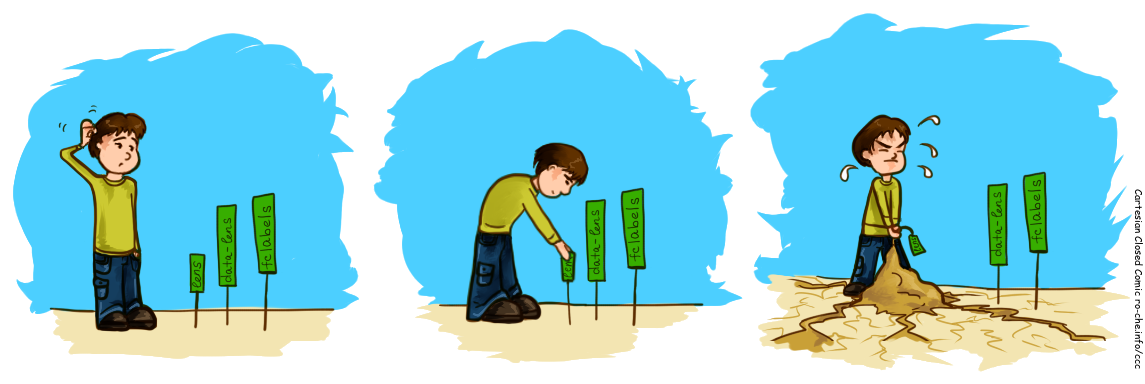
\includegraphics[width=0.9\linewidth]{images/ccc-picking-lens-library.png}
    \caption{Picking a Lens Library (Cartesian Closed Comic)}
  \end{figure}
  \begin{visibleenv}<2->
    \begin{center}
      \begin{minipage}{0.65\textwidth}
        Die von Edward Kmett natürlich! %Und nun alle:

        \visible<3->{\mintinline{bash}{$ cabal update}} \\
        \visible<4->{\mintinline{bash}{$ cabal install lens}} \\
        \visible<5->{\mintinline{bash}{Building profunctors...}} \\
        \visible<6->{\mintinline{bash}{Configuring semigroupoids...}} \\
        \visible<7->{\mintinline{bash}{Downloading kan-extensions...}}
      \end{minipage}
    \end{center}
  \end{visibleenv}
\end{frame}

\begin{frame}[t,fragile]
  \frametitle{Was sind Lenses?}
  Eine Lens beschreibt eine (feste) Position in einer Datenstruktur, an der ein Wert eines bestimmten Typs gespeichert ist.
  Mit einer Lens ist es möglich, diesen Wert auszulesen und zu überschreiben.
  \begin{columns}[t]
    \column{.45\textwidth}
    \begin{visibleenv}<2->
\begin{haskellcode*}{fontsize=\small}
data Address = Address
  { _streetLine :: String
  , _townLine :: String
  }

data Person = Person
  { _firstName :: String
  , _lastName :: String
  , _address :: Address
  }
\end{haskellcode*}
    \end{visibleenv}
    \vspace{1em}
    \column{.5\textwidth}
    \begin{visibleenv}<3->
\begin{haskellcode*}{fontsize=\small, escapeinside=||}
data Lens|\kreuz| s a = Lens|\kreuz|
  { getter :: s -> a
  , setter :: a -> s -> s
  }
\end{haskellcode*}
    \end{visibleenv}
    \begin{onlyenv}<4>
\begin{haskellcode*}{fontsize=\small, escapeinside=||}
address :: Lens|\kreuz| Person Address
address = Lens|\kreuz|
  { getter = _address
  , setter = \a p ->
      p { _address = a }
  }
\end{haskellcode*}
    \end{onlyenv}
    \begin{onlyenv}<5->
      Lens-Gesetze:
      \begin{enumerate}
        \small
        \item \haskellinline{a = getter l (setter l a s)}
        \item \haskellinline{  setter l a . setter l b} \\
        \haskellinline{= setter l a}
        \item \haskellinline{s = setter l (getter l s) s}
      \end{enumerate}
      \note{Das sind die ``costate comonad coalgebra'' Gesetze}
    \end{onlyenv}
  \end{columns}
\begin{onlyenv}<4>
\begin{haskellcode*}{fontsize=\small, escapeinside=||}
 streetLine, townLine :: Lens|\kreuz| Address String
 firstName,  lastName :: Lens|\kreuz| Person String
\end{haskellcode*}
\end{onlyenv}
\begin{onlyenv}<5->
\begin{haskellcode*}{fontsize=\small, escapeinside=||}
 streetLine, townLine :: Lens|\kreuz| Address String
 firstName,  lastName :: Lens|\kreuz| Person String
 address              :: Lens|\kreuz| Person Address
\end{haskellcode*}
\end{onlyenv}
\end{frame}

\begin{frame}[fragile]
  \frametitle{Komponieren von Lenses}
\begin{haskellcode*}{escapeinside=||}
compose :: Lens|\kreuz| s a -> Lens|\kreuz| a b -> Lens|\kreuz| s b
\end{haskellcode*}
  \vspace{-12pt}
  \begin{visibleenv}<2->
\begin{haskellcode*}{escapeinside=||}
compose l m = Lens|\kreuz|
  { getter = getter m . getter l
  , setter = \b s -> setter l (setter m b (getter l s)) s
  }
\end{haskellcode*}
  \end{visibleenv}
\begin{haskellcode*}{escapeinside=||}
personTownLine :: Lens|\kreuz| Person String
personTownLine = compose address townLine
\end{haskellcode*}

\vspace{1em}

  \begin{visibleenv}<3->
    Folgende Hilfsfunktion ist oft nützlich:
\begin{haskellcode*}{escapeinside=||}
modify :: Lens|\kreuz| s a -> (a -> a) -> s -> s
modify l f s = setter l (f (getter l s)) s
\end{haskellcode*}
    Zum Beispiel, um die Stadt in der Adresse in Versalien zu schreiben:
\begin{haskellcode*}{escapeinside=||}
person' = modify personTownLine (map toUpper) person
\end{haskellcode*}
  \end{visibleenv}
\end{frame}

\begin{frame}[fragile]
  \frametitle{
    Alles wunderbar? Leider nein
  }

  \textbf{Problem Nr. 1}: Bei der Auswertung
\begin{haskellcode*}{fontsize=\small, escapeinside=||}
  modify (compose l m) f s
= setter (compose l m) (f (getter (compose l m) s)) s
= setter l (setter m (f (getter m (getter l s))) (getter l s)) s
\end{haskellcode*}
  wird \haskellinline{getter l s} zweimal berechnet.
  Besser wäre
\begin{haskellcode*}{fontsize=\small, escapeinside=||}
  modify (compose l m) f s
= let a = getter l s in setter l (setter m (f (getter m a)) a) s
\end{haskellcode*}

  \begin{visibleenv}<2->
    \begin{columns}[t]
      \column{.43\textwidth}

      \textbf{Problem Nr. 2}: In \haskellinline{modify} wird die Datenstruktur zweimal durchlaufen: Einmal, um den gesuchten Wert zu extrahieren, dann nochmal, um den neuen Wert abzulegen. \\
      Das kann kostspielig sein, z.\,B. bei der Lens rechts.
      \column{.5\textwidth}
\begin{haskellcode*}{fontsize=\footnotesize, escapeinside=??}
data NonEmpty a =
  Cons a (NonEmpty a) | Last a
last :: Lens?\kreuz? (NonEmpty a) a
last = Lens?\kreuz? getter setter
 where
  getter (Cons _ xs) = getter xs
  getter (Last x) = x
  setter a (Cons x xs) =
    Cons x (setter a xs)
  setter a (Last _) = Last a
\end{haskellcode*}
    \end{columns}
  \end{visibleenv}
  \note{
    Man kann diese Probleme auch anders lösen: Nämlich, indem man Lenses über die Store-Komonade definiert:

\begin{haskellcode*}{}
newtype Lens a b = Lens (a -> Store b a)
data Store b a = Store (b -> a) b
\end{haskellcode*}

    Das ermöglicht, die Datenstruktur nur einmal zu durchlaufen.

    Dies macht das Paket \verb|data-lens| von Edward Kmett. (Das ist der Vorgänger seiner \verb|lens|-Library.)
  }
\end{frame}

\begin{frame}[fragile,t]
  \frametitle{
    Alles wunderbar? Leider nein
    \hfill
    {
      \small \color{greenncs}
      \visible<2->{\texttt{\{-\# LANGUAGE Rank2Types \#-\}}}
    }
  }
  \textbf{Idee}: Erweitere die Definition einer Lens um die \haskellinline{modify}-Funktion. \\
  \begin{visibleenv}<2->
    Wir verallgemeinern auch gleich \haskellinline{modify} auf effektvolle Updatefunktionen, d.\,h. solche, die beispielsweise \haskellinline{IO} verwenden:
  \end{visibleenv}
  \begin{onlyenv}<1>
\begin{haskellcode*}{escapeinside=||}
data Lens|\kkreuz| s a = Lens|\kkreuz|
  { getter  :: s -> a
  , setter  :: a -> s -> s
  , modify  ::                   (a ->   a) -> s ->   s
  }
\end{haskellcode*}
  \end{onlyenv}
  \begin{onlyenv}<2-3>
\begin{haskellcode*}{escapeinside=||}
data Lens|\kkreuz| s a = Lens|\kkreuz|
  { getter  :: s -> a
  , setter  :: a -> s -> s
  , modifyF :: |\fa| f. Functor f => (a -> f a) -> s -> f s
  }
\end{haskellcode*}
  \end{onlyenv}
  \begin{onlyenv}<4->
\begin{haskellcode*}{escapeinside=||}
data Lens|\kkreuz| s a = Lens|\kkreuz|
  { {-getter  :: s -> a
  , setter  :: a -> s -> s
  ,-} modifyF :: |\fa| f. Functor f => (a -> f a) -> s -> f s
  }
\end{haskellcode*}
  \end{onlyenv}

  \vspace{2em}

  \begin{onlyenv}<3->
    \Large Bahnbrechende Einsicht von Twan van Laarhoven: \\

    \colorbox{yellow}{
      \huge \haskellinline{modifyF} umfasst \haskellinline{getter} und \haskellinline{setter}!
    }
  \end{onlyenv}
  \note<3->{Diese Einsicht hat Twan van Laarhoven 2009 im Blogartikel \href{http://twanvl.nl/blog/haskell/cps-functional-references}{``CPS based functional references''} veröffentlicht.}
\end{frame}

\begin{frame}[fragile]
  \frametitle{
    \colorbox{yellow}{
      \haskellinline{modifyF} umfasst
      \visible<2->{{\small 1.}} \haskellinline{getter} und
      \visible<3->{{\small 2.}} \haskellinline{setter}
    }
  }

\begin{haskellcode*}{escapeinside=||}
type Lens' s a = |\fa| f. Functor f => (a -> f a) -> s -> f s
\end{haskellcode*}

  \begin{enumerate}
    \item
    \begin{visibleenv}<2->
\begin{haskellcode}
(.^) :: s -> Lens' s a -> a
\end{haskellcode}
    \end{visibleenv}
    \vspace{-0.8em}
    \begin{visibleenv}<7->
\begin{haskellcode}
s .^ l = getConst (l Const s)
\end{haskellcode}
    \end{visibleenv}

    \begin{visibleenv}<6->
\begin{haskellcode}
newtype Const a b = Const { getConst :: a }
instance Functor (Const a) where
  fmap _ (Const b) = Const b
\end{haskellcode}
    \end{visibleenv}
    \vspace{1em}

    \item
    \begin{visibleenv}<3->
\begin{haskellcode}
(.~) :: Lens' s a -> a -> s -> s
\end{haskellcode}
    \end{visibleenv}
    \vspace{-0.8em}
    \begin{visibleenv}<5->
\begin{haskellcode}
(.~) l a s = getId (l (\_ -> Id a) s)
\end{haskellcode}
    \end{visibleenv}

    \begin{visibleenv}<4->
\begin{haskellcode}
newtype Id a = Id { getId :: a }
instance Functor Id where
  fmap f (Id a) = Id (f a)
\end{haskellcode}
    \end{visibleenv}
  \end{enumerate}
\end{frame}

\begin{frame}[fragile]
  \frametitle{Komponieren von \haskellinline{Lens'}es}
  \begin{onlyenv}<1>
    \begin{tabular}{r l}
      Gegeben: & \haskellinline{ l  :: Lens' s a} \\
      und & \haskellinline{ m  :: Lens' a b} \\[0.4em]
      Gesucht: & \haskellinline{ ?  :: Lens' s b}
    \end{tabular}
  \end{onlyenv}
  \begin{onlyenv}<2>
    \begin{tabular}{r l}
      Gegeben: & \haskellinline[escapeinside=||]{ l  :: |\fa| f. Functor f => (a -> f a) ->  s -> f s} \\
      und & \haskellinline[escapeinside=||]{ m  :: |\fa| f. Functor f => (b -> f b) ->  a -> f a} \\[0.4em]
      Gesucht: & \haskellinline[escapeinside=||]{ ?  :: |\fa| f. Functor f => (b -> f b) ->  s -> f s}
    \end{tabular}
  \end{onlyenv}
  \begin{onlyenv}<3>
    \begin{tabular}{r l}
      Gegeben: & \haskellinline[escapeinside=||]{ l  :: |\fa| f. Functor f => (a -> f a) -> (s -> f s)} \\
      und & \haskellinline[escapeinside=||]{ m  :: |\fa| f. Functor f => (b -> f b) -> (a -> f a)} \\[0.4em]
      Gesucht: & \haskellinline[escapeinside=||]{ ?  :: |\fa| f. Functor f => (b -> f b) -> (s -> f s)}
    \end{tabular}
  \end{onlyenv}
  \begin{onlyenv}<4->
    \begin{tabular}{r l}
      Gegeben: & \haskellinline[escapeinside=||]{ l  :: |\fa| f. Functor f => (a -> f a) -> (s -> f s)} \\
      und & \haskellinline[escapeinside=||]{ m  :: |\fa| f. Functor f => (b -> f b) -> (a -> f a)} \\[0.4em]
      Gesucht: & \verb|l.m|\haskellinline[escapeinside=||]{ :: |\fa| f. Functor f => (b -> f b) -> (s -> f s)}
    \end{tabular}
  \end{onlyenv}

  \begin{visibleenv}<5->
    \vspace{1em}
    Dabei ist \verb|.| die stinknormale Funktionsverkettung aus der \verb|Prelude|!
    \vspace{1em}
  \end{visibleenv}

  \begin{visibleenv}<6->
    Im Beispiel vom Anfang:
\begin{haskellcode}
address :: Lens' Person Address
address f (Person first last addr) =
  fmap (Person first last) (f addr)
\end{haskellcode}
  \end{visibleenv}
  \begin{visibleenv}<7->
\begin{haskellcode}
streetLine, townLine :: Lens' Address String
firstName,  lastName :: Lens' Person String
\end{haskellcode}
  \end{visibleenv}
  \begin{visibleenv}<8->
    Dann haben wir \enspace
    \haskellinline{address.townLine :: Lens' Person String}
  \end{visibleenv}
\end{frame}

\begin{frame}[fragile,t]
  \frametitle{Was ist ein Traversal?}
\begin{haskellcode}
class (Functor t, Foldable t) => Traversable t where
  traverse :: Applicative f => (a -> f b) -> t a -> f (t b)
\end{haskellcode}
  \begin{onlyenv}<2->
    {\normalsize Ein \haskellinline{Traversal' s a} ermöglicht das Durchlaufen und Abändern von mehreren Werten vom Typ \verb|a| in einem vom Typ \verb|s| mit applik. Effekten.}
  \end{onlyenv}
  \begin{onlyenv}<3->
\begin{haskellcode}
type Traversal' s a = forall f.
  Applicative f => (a -> f a) -> s -> f s
\end{haskellcode}
\begin{haskellcode}
traverse :: Traversable t => Traversal' (t a) a
\end{haskellcode}
  \end{onlyenv}
  \begin{onlyenv}<4->
\begin{haskellcode}
evenIxs :: Traversal' [a] a
evenIxs f [] = pure []
evenIxs f [x] = (:[]) <$> f x
evenIxs f (x:y:xs) = (\x' xs' -> x':y:xs')
                     <$> f x <*> evenIxs f xs
\end{haskellcode}
  \end{onlyenv}
  \begin{onlyenv}<4->
    Traversals lassen sich wie Lenses verknüpfen:
\begin{haskellcode}
(.) :: Traversal' s a -> Traversal' a b -> Traversal' s b
\end{haskellcode}
  \end{onlyenv}
\end{frame}

\begin{frame}[fragile]
  \frametitle{Wiederholung}
  Eine \haskellinline{Lens' s a} gibt Lese- und Schreibzugriff auf ein \haskellinline{a} innerhalb eines \haskellinline{s}.

  Ein \haskellinline{Traversal' s a} iteriert über kein, ein oder mehrere \haskellinline{a} innerhalb eines \haskellinline{s} (mit R/W-Zugriff).

\begin{haskellcode*}{fontsize=\small,escapeinside=||}
type Lens'      s a = |\fa| f.     Functor f => (a -> f a) -> s -> f s
type Traversal' s a = |\fa| f. Applicative f => (a -> f a) -> s -> f s
\end{haskellcode*}

  Lenses sowie Traversals lassen sich mit der normalen Funktionskomposition \verb|(.)| verketten.

\begin{haskellcode}
(.^) :: s -> Lens' s a -> a
(.~) :: Lens' s a -> a -> s -> s
\end{haskellcode}
\end{frame}

\begin{frame}[t,fragile]
  \frametitle{Weitere optische Gerätschaften aus \haskellinline{lens}}
  \begin{center}
    \begin{tikzpicture}[
        overlay,
        myrect/.style={
          rectangle,
          draw,
          rounded corners,
          inner sep=4pt
        }
      ]
      \begin{scope}[shift={(1,0)}]
        %\draw[use as bounding box] (-5,-1) rectangle (2.5,1.5);
        \node<7->[myrect] (setter) at (-4,0.5) {Setter};
        \node<6->[myrect] (fold) at (-4,-0.5) {Fold};
        \node<2->[myrect] (traversal) at (-2,0.5) {Traversal};
        \node<5->[myrect] (getter) at (-2,-0.5) {Getter};
        \node<3->[myrect] (prism) at (0,0.5) {Prism};
        \node[myrect] (lens) at (0,-0.5) {Lens};
        \node<4->[myrect] (iso) at (1.5,0) {Iso};
        \draw<7->[->] (setter) -- (traversal);
        \draw<6->[->] (fold) -- (traversal);
        \draw<6->[->] (fold) -- (getter);
        \draw<2->[->] (traversal) -- (lens);
        \draw<3->[->] (traversal) -- (prism);
        \draw<5->[->] (getter) -- (lens);
        \draw<4->[->] (prism) -- (iso);
        \draw<4->[->] (lens) -- (iso);
      \end{scope}
    \end{tikzpicture}
  \end{center}

  \vspace{2em}

  {
  \setbeamercolor{alerted text}{fg=orange}
  \setbeamerfont{alerted text}{series=\mdseries}

  \begin{onlyenv}<1-7>
    \begin{tabular}{r l}
      \visible<7->{\alert<7>{Setter}} &
      \visible<7->{in \haskellinline{s} gibt es veränderbare \haskellinline{a}'s} \\

      \visible<6->{\alert<6>{Fold}} &
      \visible<6->{Funktion \haskellinline{s -> [a]}} \\

      \visible<5->{\alert<5>{Getter}} &
      \visible<5->{Funktion \haskellinline{s -> a}} \\

      \visible<2->{\alert<2>{Traversal}} &
      \visible<2->{ein \haskellinline{s} besteht aus \haskellinline{a}'s und anderen Daten} \\

      \alert<1>{Lens} &
      ein \haskellinline{s} besteht aus einem \haskellinline{a} und anderen Daten \\

      \visible<3->{\alert<3>{Prism}} &
      \visible<3->{ein \haskellinline{s} ist ein \haskellinline{a} oder etwas anderes} \\

      \visible<4->{\alert<4>{Iso}} &
      \visible<4->{ein \haskellinline{s} ist dasselbe wie ein \haskellinline{a}}
    \end{tabular}
  \end{onlyenv}}

  \begin{onlyenv}<8->
    \vspace{-0.7em}
\begin{haskellcode*}{fontsize=\footnotesize,baselinestretch=1.2}
   Setter' s a =                                (a -> Id a) -> s -> Id s
     Fold  s a = (Contrav't f, Applicative f) => (a -> f a) -> s -> f s
   Getter  s a =     (Contrav't f, Functor f) => (a -> f a) -> s -> f s
Traversal' s a =               Applicative f  => (a -> f a) -> s -> f s
     Lens' s a =                   Functor f  => (a -> f a) -> s -> f s
    Prism' s a =    (Choice p, Applicative f) =>  p a (f a) -> p s (f s)
      Iso' s a =    (Profunctor p, Functor f) =>  p a (f a) -> p s (f s)
\end{haskellcode*}
  \end{onlyenv}

  % Lens-Beispiele
  \begin{onlyenv}<1>
\begin{haskellcode*}{fontsize=\small}
lens :: (s -> a) -> (s -> a -> s) -> Lens' s a
_1 :: Lens' (x,y) x     _1 :: Lens' (x,y,z) x
_2 :: Lens' (x,y) y     _2 :: Lens' (x,y,z) y
choosing :: Lens' s a -> Lens' s' a -> Lens' (Either s s') a
inside :: Lens' s a -> Lens' (e -> s) (e -> a)
devoid :: Lens' Void a    united :: Lens' a ()
\end{haskellcode*}
  % -- Void = (a, Void)
  % -- a    = (a, ())
  \end{onlyenv}

  % Traversal-Beispiele
  \begin{onlyenv}<2>
\begin{haskellcode*}{fontsize=\small}
traverse :: Traversable t => Traversal' (t a) a
both :: Traversal' (s,s) s
beside :: Traversal' s a -> Traversal s' a -> Traversal' (s,s') a
taking :: Int -> Traversal' s a -> Traversal' s a
ignored :: Traversal' s a -- trivial traversal
\end{haskellcode*}
  \end{onlyenv}

  % Prism-Beispiele
  \begin{onlyenv}<3>
\begin{haskellcode*}{fontsize=\small}
prism :: (a -> s) -> (s -> Either s a) -> Prism' s a
_Left :: Prism' (Either a c) a    _Right :: Prism' (Either a c) c
_Just :: Prism' (Maybe a) a
_Void :: Prism' s Void
outside :: Prism' s a -> Lens' (s -> r) (a -> r)
\end{haskellcode*}
  \end{onlyenv}

  % Iso-Beispiele
  \begin{onlyenv}<4>
\begin{haskellcode}
iso :: (s -> a) -> (a -> s) -> Iso' s a
curried :: Iso' ((a, b) -> c) (a -> b -> c)
packed :: Iso' String Text
from :: Iso' s a -> Iso' a s
mapping :: Functor f => Iso' s a -> Iso' (f s) (f a)
\end{haskellcode}
  \end{onlyenv}

  % Getter-Beispiele
  \begin{onlyenv}<5>
\begin{haskellcode}
to :: (s -> a) -> Getter s a
to length :: Getter [a] Int
\end{haskellcode}
  \end{onlyenv}

  % Fold-Beispiele
  \begin{onlyenv}<6>
\begin{haskellcode}
unfolded :: (b -> Maybe (a, b)) -> Fold b a
folding :: Foldable f => (s -> f a) -> Fold s a
folded  :: Foldable f => Fold (f a) a
replicated :: Int -> Fold a a
\end{haskellcode}
  \end{onlyenv}

  % Setter-Beispiele
  \begin{onlyenv}<7>
\begin{haskellcode}
sets :: ((a -> a) -> s -> s) -> Setter' s a
mapped :: Functor f => Setter' (f a) a
mapped :: Setter' (x -> a) a
\end{haskellcode}
  \end{onlyenv}

  {\small
  \begin{onlyenv}<9->
    \begin{itemize}
      \item<9-> Durch Subtyping ist jeder Iso eine Lens, jedes Prism ein Traversal \ldots
      \item<10-> Man kann z.\,B. eine Lens mit einem Traversal verknüpfen (mit \haskellinline{.}) und man bekommt ein Traversal.
      \item<11-> Viele Beispielfunktionen haben einen allgemeineren Typ als angegeben.
    \end{itemize}
  \end{onlyenv}}

  \note{Prismen sind dual zu Lenses: Während eine \haskellinline{Lens' s a} den Typ \verb|s| als Produkt von \verb|a| und einem zweiten Typ darstellt, gibt ein \haskellinline{Prism' s a} eine Darsellung von \verb|s| als Summe von \verb|a| und einem zweiten Typ an.}
  \note{Es gibt außerdem noch den Typ \haskellinline{Review t b}. Er entspricht einer Funktion \haskellinline{b -> t}. Unter der Dualität von \haskellinline{Lens'} und \haskellinline{Prism'} entspricht ein \haskellinline{Getter} einem \haskellinline{Review}. Insbesondere ist jedes \haskellinline{Prism' b t} ein \haskellinline{Review t b}.}

  \note{\url{https://github.com/ekmett/lens/wiki/Derivation}{Das Lens-Wiki beschreibt} die Herleitung dieser Typen.}
\end{frame}

{\setbeamertemplate{background}{}
\begin{frame}
  % Quelle: https://ro-che.info/ccc/29
  \begin{center}
    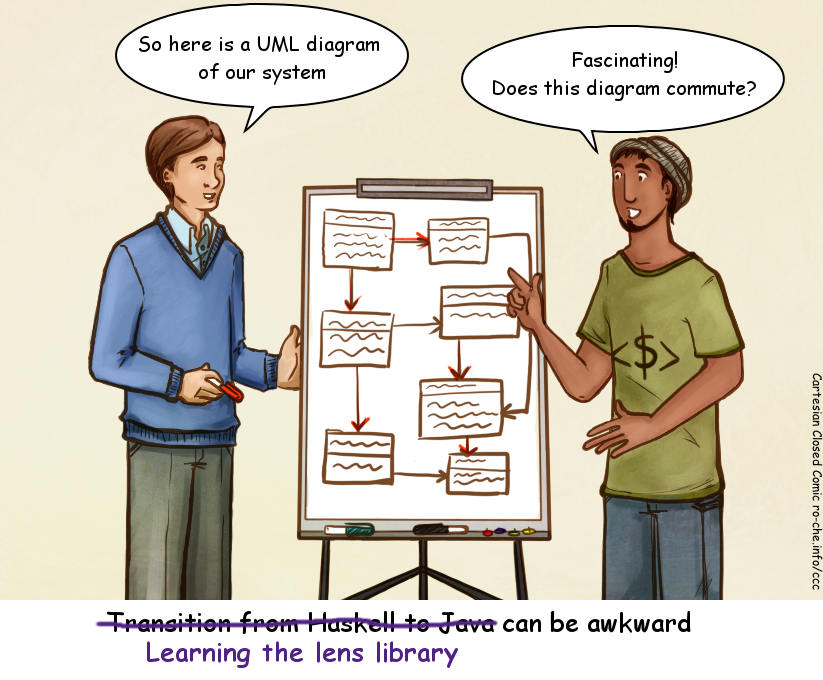
\includegraphics[width=0.9\linewidth]{images/ccc-does-diagram-commute.jpg}
  \end{center}
\end{frame}}

\begin{frame}[fragile,t]
  \frametitle{Polymorphe Updates}
  \begin{onlyenv}<1-6>
\begin{haskellcode*}{escapeinside=||}
type Lens s t a b = forall f.
  Functor f => (a -> f b) -> s -> f t
\end{haskellcode*}
  \end{onlyenv}
  \begin{onlyenv}<2-6>
\begin{haskellcode*}{escapeinside=||}
type Lens' s a = Lens s s a a
\end{haskellcode*}
  \end{onlyenv}
  \begin{onlyenv}<3-6>
\begin{haskellcode*}{escapeinside=||}
_1 :: Lens (x,y) (x',y) x x'
\end{haskellcode*}
  \end{onlyenv}
  \begin{onlyenv}<4-6>
\begin{haskellcode*}{escapeinside=||}
  set (_2._1) 42 ("hello",("world","!!!"))
|\ev| ("hello",(42,"!!!"))
\end{haskellcode*}
  \end{onlyenv}
  \begin{onlyenv}<7->
\begin{haskellcode*}{escapeinside=||}
type Prism s t a b = forall p f.
  (Choice p, Applicative f) => p a (f b) -> p s (f t)
\end{haskellcode*}
\begin{haskellcode*}{escapeinside=||}
type Prism' s a = Prism s s a a
\end{haskellcode*}
\begin{haskellcode*}{escapeinside=||}
_Right :: Prism (Either x y) (Either x y') y y'
\end{haskellcode*}
\begin{haskellcode*}{escapeinside=||}
  set (_Right._2) "world" (Right ("hello",42))
|\ev| Right ("hello","world")
\end{haskellcode*}
  \end{onlyenv}
  \begin{onlyenv}<5->
\begin{haskellcode*}{escapeinside=||}
type Setter s t a b = (a -> Id b) -> (s -> Id t)
type Setter' s a = Setter s s a a
mapped :: Functor f => Setter (f x) (f y) x y
\end{haskellcode*}
  \end{onlyenv}
  \begin{onlyenv}<6->
\begin{haskellcode*}{escapeinside=||}
type Traversal s t a b = forall f.
  Applicative f => (a -> f b) -> (s -> f t)
type Traversal' s a = Traversal s s a a
traverse :: Traversable t => Traversal (t x) (t y) x y
\end{haskellcode*}
  \end{onlyenv}
  \note{Polymorphe Updates wurden zum ersten Mal 2012 in \href{http://r6.ca/blog/20120623T104901Z.html}{einem Blogartikel} von Russell O'Connor beschrieben.}
\end{frame}

\begin{frame}
  \frametitle{Beispiel: Curry-Feed parsen}
  \begin{center}
    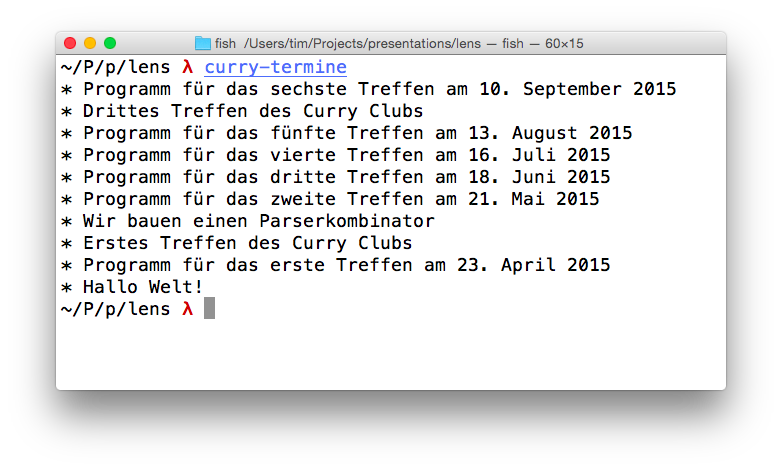
\includegraphics[width=10cm]{images/curry-termine-screenshot.png}
  \end{center}
\end{frame}

\begin{frame}
  \frametitle{Beispiel: Curry-Feed parsen}
  \inputminted[fontsize=\footnotesize]{xml}{curry-feed.xml}
\end{frame}

{\setbeamertemplate{background}{}
\begin{frame}[fragile,b]
  \frametitle{Beispiel: Curry-Feed parsen}
  \inputminted[fontsize=\small]{haskell}{curry-termine/Main.hs}
  \note{Verwendete Packages: \verb|lens|, \verb|text|, \verb|xml-conduit|, \verb|wreq|, \verb|xml-lens|}
  \note{Es gibt auch Lenses für JSON-Daten. Diese waren früher in \verb|lens| enthalten, jetzt sind sie Teil des Pakets \verb|lens-aeson|.}
  \begin{visibleenv}<2->
    \vspace{-7cm}
    \hfill \begin{minipage}{0.55 \linewidth}
      \begin{mdframed}[backgroundcolor=yellow]
\begin{haskellcode*}{fontsize=\footnotesize}
responseBody
  :: Lens' (Response body) body
root :: Lens' Document Element
nodes :: Lens' Element [Node]
_Element :: Prism' Node Element
named :: CI Text
      -> Traversal' Element Element
text :: Traversal' Element Text
\end{haskellcode*}
      \end{mdframed}
    \end{minipage}
  \end{visibleenv}
  \begin{visibleenv}<3->
    \vspace{-2cm}
    \begin{center}
      
\includegraphics[height=3cm]{images/lens-jquery.png}
    \end{center}
    \vspace{8cm}
  \end{visibleenv}
\end{frame}
}

\begin{frame}[fragile,t]
  \frametitle{Wie bekomme ich Lenses für meine Datentypen?}
  \vspace{-1.2em}
  \begin{columns}[t]
    \column{0.48\textwidth}
    \begin{onlyenv}<1-2>
      \begin{visibleenv}<2>
\begin{haskellcode*}{stripnl=false,fontsize=\small}
{-# LANGUAGE Rank2Types #-}
-- keine Imports nötig

\end{haskellcode*}
      \end{visibleenv}
    \end{onlyenv}
    \begin{onlyenv}<3>
\begin{haskellcode*}{stripnl=false,fontsize=\small}
{-# LANGUAGE TemplateHaskell #-}
import Control.Lens.TH

\end{haskellcode*}
    \end{onlyenv}
    \begin{onlyenv}<4>
\begin{haskellcode*}{stripnl=false,fontsize=\small}
{-# LANGUAGE TemplateHaskell #-}
import Lens.Micro.TH
-- aus 'microlens-th' (Beispiel)
\end{haskellcode*}
    \end{onlyenv}
    \begin{onlyenv}<5>
\begin{haskellcode*}{stripnl=false,fontsize=\small}
{-# LANGUAGE DeriveDataTypeable #-}
import Data.Data

\end{haskellcode*}
    \end{onlyenv}
    \begin{onlyenv}<1-4>
\begin{haskellcode*}{fontsize=\small}
data Address = Address {...}

data Person = Person
  { _firstName :: String
  , _lastName :: String
  , _address :: Address
  }
\end{haskellcode*}
    \end{onlyenv}
    \begin{onlyenv}<5>
\begin{haskellcode*}{fontsize=\small}
data Address = Address {...}
  deriving (Typeable, Data)
data Person = Person
  { _firstName :: String
  , _lastName :: String
  , _address :: Address
  } deriving (Typeable, Data)
\end{haskellcode*}
    \end{onlyenv}
    \begin{onlyenv}<2>
\begin{haskellcode*}{fontsize=\small}
address :: forall f. Functor f
        => (Address -> f Address)
        -> Person -> f Person
address f (Person first last addr) =
  fmap (Person first last) (f addr)
{-# INLINE address #-} -- empfohlen
-- und so weiter ...
\end{haskellcode*}
    \end{onlyenv}
    \begin{onlyenv}<3-4>
\begin{haskellcode*}{fontsize=\small}
makeLenses ''Address
makeLenses ''Person
\end{haskellcode*}
    \end{onlyenv}
    \begin{onlyenv}<5>
      \vspace{1em}
\begin{haskellcode*}{fontsize=\footnotesize, escapeinside=||}
-- Im Client-Code: Importiere Lens
import Data.Data.Lens
-- und benutze dann die Funktion:
biplate :: (Data s, Typeable a)
        => Traversal' s a
biplate :: Traversal' Person Address
\end{haskellcode*}
    \end{onlyenv}

    \column{.52\textwidth}
    %Drei Optionen:
    \begin{enumerate}
      \item<2-> Lenses selber schreiben \\[0.2em]
      {\small \color{dimgray}
      Vorteil: Keine Library benötigt! \\
      Nachteil: Boilerplate-Code}
      \note{Im Lens-Wiki auf \lenswithoutdep wird erklärt, wie man Lenses, Traversals, Folds etc. schreiben kann, ohne auf Lens zu dependen.}
      \item<3-> Lenses generieren mit Template Haskell-Funktionen aus \haskellinline{lens} \\[0.2em]
      {\small \color{dimgray}
      Vorteil: Komfortabel \\
      Nachteil: Template Haskell}
      \item<4-> Lenses generieren mit einer anderen Bibliothek und TH \\[0.2em]
      {\small \color{dimgray}
      Vorteil: Komfortabel, keine Dependency auf \verb|lens| \\
      Nachteil: Template Haskell}
      \item<5-> Derive \verb|Data| und \verb|Typeable| und benutze \verb|Data.Data.Lens| \\[0.2em]
      {\small \color{dimgray}
      Nachteil: nur typgesteuerte Traversals möglich}
    \end{enumerate}
  \end{columns}
  \note{Lenses bieten die Möglichkeit, die konkrete Implementierung eines Datentyps nach außen hin zu verstecken, aber dennoch Zugriff auf Felder zu gewähren. Dadurch gewinnt man die Freiheit, die Implementierung des Datentyps zu verbessern, ohne das Interface nach außen zu verändern.}
  \note{\verb|Data.Data.Lens| und \verb|Control.Lens.Plated| basieren auf der \verb|uniplate|-Library für generisches Programmieren von Neil Mitchell.}
  \note{Die Plated-Funktionalität von Lens kann besonders hilfreich für Compiler-Programmierer sein: Damit kann man nämlich z.B. mit wenig Code auf einem AST Transformationen durchführen.}
\end{frame}

{\setbeamertemplate{background}{
\includegraphics[width=\paperwidth,height=\paperheight,keepaspectratio]{images/donald-detective-wolle-bg.jpg}}
\setlength{\fboxsep}{2pt} % kaum Innenabstand in \colorbox'en
\begin{frame}
  \frametitle{Beispiel: Imperative (Spiele-) Programmierung}
  \begin{center}
    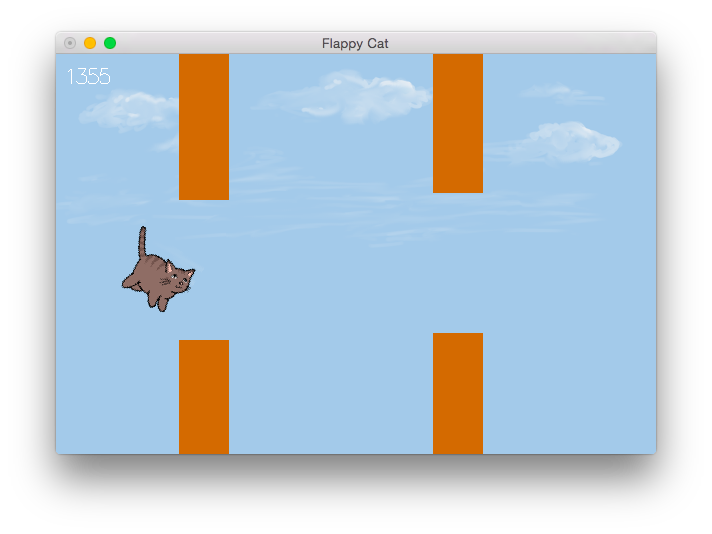
\includegraphics[width=10cm]{images/flappy-cat-screenshot.png}
  \end{center}
\end{frame}

\begin{frame}[fragile]
  \frametitle{Beispiel: Imperative (Spiele-) Programmierung}
\begin{haskellcode}
data Pos = Pos { _x :: Float, _y :: Float }
makeLenses ''Pos

newtype Hurdle = Hurdle { _hurdlePos :: Pos }
makeLenses ''Hurdle

data GameState = Running | Paused | GameOver

data FlappyCat =
  FlappyCat
  { _gen :: StdGen
  , _gameState :: GameState
  , _catPos :: Pos
  , _velY :: Float
  , _hurdles :: [Hurdle]
  }
makeLenses ''FlappyCat
\end{haskellcode}
\end{frame}

\begin{frame}[fragile]
  \frametitle{Beispiel: Imperative (Spiele-) Programmierung}
    Ein paar Hilfsfunktionen:
\begin{haskellcode}
randomHurdle :: (RandomGen g, MonadState g m)
             => Float -> m Hurdle
passes :: Pos -> Hurdle -> Bool
catExtremePoints :: FlappyCat -> [Pos]
\end{haskellcode}

  \vspace{1em}
  \begin{visibleenv}<2->
    Eine Monade:
\begin{haskellcode}
type FlappyMonad = ContT () (State FlappyCat)

execFlappyMonad :: FlappyMonad () -> FlappyCat -> FlappyCat
execFlappyMonad = execState . flip runContT return

abort :: FlappyMonad ()
abort = ContT $ const $ return ()
\end{haskellcode}
  \end{visibleenv}
\end{frame}

\begin{frame}[b,fragile]
  \frametitle{Beispiel: Imperative (Spiele-) Programmierung}
\begin{haskellcode*}{escapeinside=||}
handleInput :: Event -> FlappyMonad ()
handleInput (EventKey (Char 'p') Down _ _) =
  gameState |\hl{\%=}\marktikz{t1}| \case
    Running  -> Paused
    Paused   -> Running
    GameOver -> GameOver
handleInput (EventKey (SpecialKey key) Down _ _)
  |\textbar| key `elem` jumpKeys = do
  velY |\hl{.=}\marktikz{t2}| jumpVel
  oldState <- gameState |\hl{<<.=}\marktikz{t3}| Running
  when (oldState == GameOver) $ do
    catPos.x |\hll{.=}| 0
    catPos.y |\hll{.=}| 0
    hurdles  |\hll{.=}| []
handleInput _ = return ()
\end{haskellcode*}
  % Achtung: Man muss 2x kompilieren, damit die Positionen richtig sind!
  \begin{visibleenv}<2->
    {\small
    \begin{tikzpicture}[remember picture, overlay]
      \draw[typeline] (t1) |- + (2.5, 0.3) node[typebox, anchor=north west] {\verb|:: MonadState s m|\\\verb|=> Setter' s a -> (a -> a) -> m ()|};
      \draw[typeline] (t2) |- + (4.75, -0.1) node[typebox, anchor=south west] {\verb|:: MonadState s m|\\\verb|=> Setter' s a -> a -> m ()|};
      \draw[typeline] (t3) |- + (1.5, -0.1) node[typebox, anchor=north west] {\verb|:: MonadState s m|\\\verb|=> Lens' s a -> a -> m a|};
    \end{tikzpicture}}
  \end{visibleenv}
\end{frame}

\begin{frame}[fragile]
  \frametitle{Beispiel: Imperative (Spiele-) Programmierung}
\begin{haskellcode*}{escapeinside=||}
step :: Float -> FlappyMonad ()
step dt = do
  state <- |\hl{use}\marktikz{t4}| gameState
  when (state /= Running) abort
  vy <- velY |\hl{<+=}\marktikz{t5}| dt*gravity
  px <- catPos.x |\hll{<+=}| dt*velX
  py <- catPos.y |\hll{<+=}| dt*vy
  when (py <= -h/2) $ gameState |\hll{.=}| GameOver
  hs <- hurdles |\hl{<\%=}\marktikz{t6}| filter ((> (px-w)) . (^.hurdlePos.x))
  let lastX = fromMaybe (d+w) $
        |\hll{lastOf}| (traverse.hurdlePos.x) hs
  when (lastX < px + 2*w) $ do
    hurdle <- lift $ |\hl{zoom}\marktikz{t7}| gen $ randomHurdle lastX
    hurdles |\hll{.=}| hs ++ [hurdle]
  eps <- |\hll{use}| $ to catExtremePoints
  unless (all id $ passes <$> eps <*> hs) $
    gameState |\hll{.=}| GameOver
\end{haskellcode*}
  \begin{visibleenv}<2->
    {\small
    \begin{tikzpicture}[remember picture, overlay]
      \draw[typeline] (t4) |- + (5, 0.5) node[typebox, anchor=south west] {\verb|:: MonadState s m|\\\verb|=> Getter s a -> m a|};
      \draw[typeline] (t5) |- + (3.5, 0.25) node[typebox, anchor=south west] {\verb|:: (MonadState s m, Num a)|\\\verb|=> Lens' s a -> a -> m a|};
      \draw[typeline] (t6) |- + (2, 0.85) node[typebox, anchor=south west] {\verb|:: MonadState s m|\\\verb|=> Lens' s a -> (a -> a) -> m a|};
      \draw[typeline] (t7) |- + (1, -0.1) node[typebox, anchor=north west] {\verb|:: Monad m => Lens' s t|\\\verb|-> StateT t m a -> StateT s m a|};
    \end{tikzpicture}}
  \end{visibleenv}
\end{frame}

\begin{frame}[fragile]
  \frametitle{Operatoren in Lens}

  \begin{onlyenv}<1>
\begin{haskellcode*}{fontsize=\small}
   (%~) :: Setter s t a b -> (a -> b) -> s ->     t
  (<%~) :: Lens   s t a b -> (a -> b) -> s -> (b, t)
 (<<%~) :: Lens   s t a b -> (a -> b) -> s -> (a, t)
   (%=) :: MonadState s m => Setter s s a b -> (a -> b) -> m ()
  (<%=) :: MonadState s m => Lens   s s a b -> (a -> b) -> m b
 (<<%=) :: MonadState s m => Lens   s s a b -> (a -> b) -> m a
\end{haskellcode*}
  \end{onlyenv}

  \begin{onlyenv}<2>
\begin{haskellcode*}{fontsize=\small}
   (.~) :: Setter s t a b -> b -> s ->     t
  (<.~) :: Setter s t a b -> b -> s -> (b, t)
 (<<.~) :: Lens   s t a b -> b -> s -> (a, t)
   (.=) :: MonadState s m => Setter s s a b -> b -> m ()
  (<.=) :: MonadState s m => Setter s s a b -> b -> m b
 (<<.=) :: MonadState s m => Lens'  s s a b -> b -> m a
\end{haskellcode*}
  \end{onlyenv}

  \begin{onlyenv}<3>
\begin{haskellcode*}{fontsize=\small}
   (+~) ::  Num a => Setter s t a a -> a -> s ->     t
  (<+~) ::  Num a => Lens   s t a a -> a -> s -> (a, t)
 (<<+~) ::  Num a => Lens   s t a a -> a -> s -> (a, t)
   (+=) :: (Num a, MonadState s m) => Setter' s a -> a -> m ()
  (<+=) :: (Num a, MonadState s m) => Lens'   s a -> a -> m a
 (<<+=) :: (Num a, MonadState s m) => Lens'   s a -> a -> m a
\end{haskellcode*}
  \end{onlyenv}

  \begin{onlyenv}<4>
\begin{haskellcode*}{fontsize=\small}
  (<>~) ::  Monoid a => Setter s t a a -> a -> s ->     t
 (<<>~) ::  Monoid a => Lens   s t a a -> a -> s -> (a, t)
(<<<>~) ::  Monoid a => Lens   s t a a -> a -> s -> (a, t)
  (<>=) :: (Monoid a, MonadState s m) => Setter' s a -> a -> m ()
 (<<>=) :: (Monoid a, MonadState s m) => Lens'   s a -> a -> m a
(<<<>=) :: (Monoid a, MonadState s m) => Lens'   s a -> a -> m a
\end{haskellcode*}
  \end{onlyenv}

  \begin{onlyenv}<5->
\begin{haskellcode*}{fontsize=\small}
  (||~) :: Setter s t Bool Bool -> Bool -> s ->        t
 (<||~) :: Lens   s t Bool Bool -> Bool -> s -> (Bool, t)
(<<||~) :: Lens   s t Bool Bool -> Bool -> s -> (Bool, t)
  (||=) :: MonadState s m => Setter' s Bool -> Bool -> m ()
 (<||=) :: MonadState s m => Lens'   s Bool -> Bool -> m Bool
(<<||=) :: MonadState s m => Lens'   s Bool -> Bool -> m Bool
\end{haskellcode*}
  \end{onlyenv}

  \vspace{0.25em}
  \small
  \begin{center}
    {\setlength\extrarowheight{3pt}
    \begin{tabular}{r!{\color{gray}\vrule} r r r r r}
      Funktional & \verb|%~| & \verb|.~| & \verb|+~| & \verb|<>~| & \verb?||~? \\
      Funktional mit Ergebnis & \verb|<%~| & \verb|<.~| & \verb|<+~| & \verb|<<>~| & \verb?<||~? \\
      Funktional mit vorh. Wert & \verb|<<%~| & \verb|<<.~| & \verb|<<+~| & \verb|<<<>~| & \verb?<<||~? \\ \arrayrulecolor{gray}\hline
      Monadisch & \verb|%=| & \verb|.=| & \verb|+=| & \verb|<>=| & \verb?||=? \\
      Monadisch mit Ergebnis & \verb|<%=| & \verb|<.=| & \verb|<+=| & \verb|<<>=| & \verb?<||=? \\
      Monadisch mit vorh. Wert & \verb|<<%=| & \verb|<<.=| & \verb|<<+=| & \verb|<<<>=| & \verb?<<||=? \\
    \end{tabular}}
  \end{center}

  \vspace{0.75em}
  {\small (Vollständige Liste auf \url{https://github.com/ekmett/lens/wiki/Operators})}

  \begin{visibleenv}<6->
    \vspace{-6cm}
    \begin{center}
      
\includegraphics[height=4cm]{images/lens-perl.png}
    \end{center}
    \vspace{2cm}
  \end{visibleenv}
\end{frame}
}

\begin{frame}[fragile]
  \frametitle{Beispiel: \texttt{diagrams-rubiks-cube}}
  \emph{Ziel:} Zauberwürfel und Lösungsalgorithmen zeichnen. \emph{Beispiel:}\\[1em]
  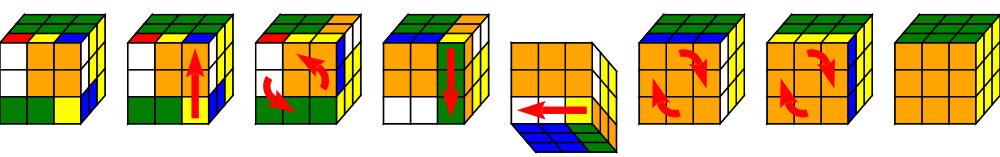
\includegraphics[width=0.65\linewidth]{images/rubiks-sequence.png}\\
  \begin{haskellcode}
import Diagrams.RubiksCube
import Control.Lens

diagram :: RubiksCubeBackend n b => Diagram b
diagram =
  let moves    = [B, R, F', R', D', F, F]
      endPos   = solvedRubiksCube
      settings = with & showStart .~ True
  in drawMovesBackward settings endPos moves
  \end{haskellcode}
\end{frame}

\begin{frame}[fragile]
  \frametitle{Beispiel: \texttt{diagrams-rubiks-cube}}

  \begin{haskellcode}
data Side a = Side
  {    _topLeft :: a,    _topCenter :: a,    _topRight :: a
  , _middleLeft :: a, _middleCenter :: a, _middleRight :: a
  , _bottomLeft :: a, _bottomCenter :: a, _bottomRight :: a
  } deriving (Show, Eq, Functor, Foldable, Traversable)
instance Applicative Side
makeLenses ''Side
  \end{haskellcode}
  \vspace{0.5em}
  \begin{minipage}{0.22 \linewidth}
    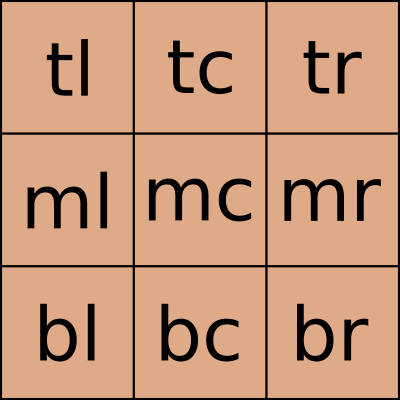
\includegraphics[width=2.25cm]{images/side.png}
  \end{minipage}
  \begin{minipage}{0.75 \linewidth}
    \begin{haskellcode}
rotCW, rotCCW :: Side a -> Side a
rotCW (Side tl tc tr ml mc mr bl bc br) =
       Side bl ml tl bc mc tc br mr tr

type Aut a = Iso' a a
rotateSideCW, rotateSideCCW :: Aut (Side a)
rotateSideCW  = iso rotCW  rotCCW
rotateSideCCW = iso rotCCW rotCW
    \end{haskellcode}
  \end{minipage}
\end{frame}

\begin{frame}[fragile]
  \frametitle{Beispiel: \texttt{diagrams-rubiks-cube}}
  \begin{haskellcode*}{fontsize=\small}
data Cube a = Cube
  { _frontSide :: a,  _backSide :: a
  ,  _leftSide :: a, _rightSide :: a
  ,    _upSide :: a,  _downSide :: a
  } deriving (Show, Eq, Functor, Foldable, Traversable)

instance Applicative Cube
makeLenses ''Cube


  \end{haskellcode*}
  %\vspace{0.5em}
  \begin{minipage}{0.3 \linewidth}
    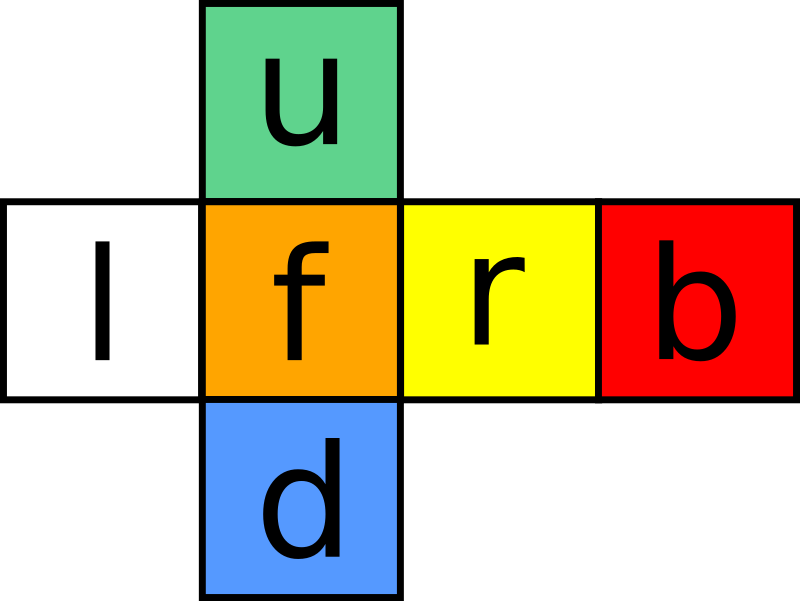
\includegraphics[width=3cm]{images/cube.png}
  \end{minipage}
  \begin{minipage}{0.67 \linewidth}
    \begin{haskellcode*}{fontsize=\small}
rotRight', rotLeft' :: Cube a -> Cube a
rotRight' (Cube f b l r u d) =
           Cube l r b f u d

rotateRight', rotateLeft' :: Aut (Cube a)
rotateRight' = iso rotRight' rotLeft'
rotateLeft'  = iso rotLeft'  rotRight'
    \end{haskellcode*}
  \end{minipage}
\end{frame}

\begin{frame}[fragile]
  \frametitle{Beispiel: \texttt{diagrams-rubiks-cube}}
  \begin{minipage}{0.43 \linewidth}
    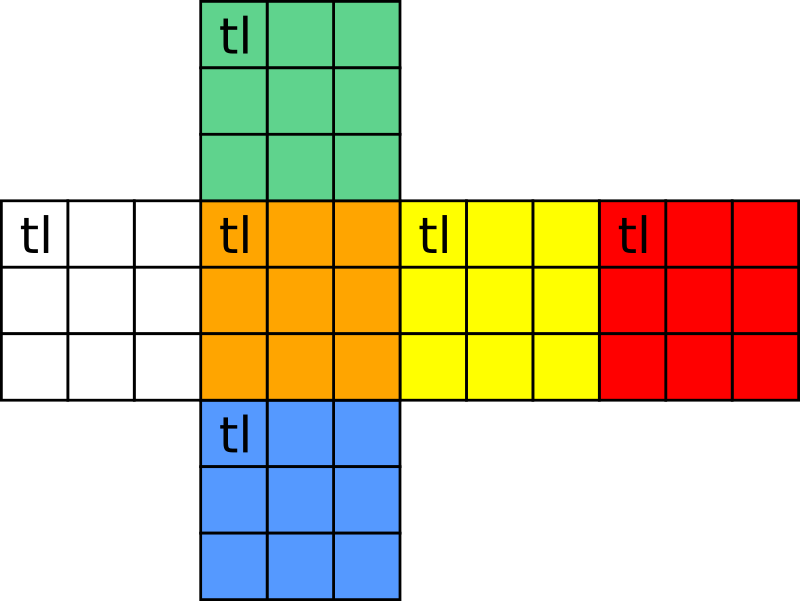
\includegraphics[width=4.5cm]{images/rubikscube.png}
  \end{minipage}
  \begin{minipage}[b]{0.55 \linewidth}
    \begin{haskellcode*}{fontsize=\small}
newtype RubiksCube a = RubiksCube
  { _cube :: Cube (Side a) }
    deriving (Show, Eq, Functor)

instance Applicative RubiksCube
makeLenses ''RubiksCube
    \end{haskellcode*}
  \end{minipage}
\end{frame}

\begin{frame}[fragile]
  \frametitle{Beispiel: \texttt{diagrams-rubiks-cube}}
  %-- | Rotate the whole Rubik's Cube such that the front
  %-- side becomes the new right side and the top and
  %-- bottom sides stay fixed.
  \begin{haskellcode}
-- Wende einen Automorphismus auf alle Komponenten an
cong :: Traversal' s a -> Aut a -> Aut s
cong t i = withIso i $ \f g -> iso (over t f) (over t g)

rotateRight, rotateLeft :: Aut (RubiksCube a)
rotateRight =
  cong cube $ rotateRight'
            . cong   upSide rotateSideCCW
            . cong downSide rotateSideCW
rotateLeft = from rotateRight

rotateUp, rotateDown :: Aut (RubiksCube a)

rotateCW, rotateCCW :: Aut (RubiksCube a)
rotateCW  = rotateUp . rotateLeft . rotateDown
rotateCCW = from rotateCW
  \end{haskellcode}
  % TODO: Skizze von der Wirkung von rotateRight
\end{frame}

\begin{frame}[fragile]
  \frametitle{Beispiel: \texttt{diagrams-rubiks-cube}}
  \begin{haskellcode*}{fontsize=\small}
data Vec4 a = Vec4 a a a a
  deriving (Show, Eq, Functor, Foldable, Traversable)

cycRight, cycLeft :: Vec4 a -> Vec4 a
cycRight (Vec4 a b c d) = Vec4 d a b c

cycleRight, cycleLeft :: Aut (Vec4 a)
cycleRight = iso cycRight cycLeft
cycleLeft  = from cycleRight

liftVec4 :: Lens' s a -> Lens' (Vec4 s) (Vec4 a)
liftVec4 l = lens getter setter
  where
    getter = fmap (^. l)
    setter (Vec4 a b c d) (Vec4 a' b' c' d') =
      Vec4 (set l a' a) (set l b' b) (set l c' c) (set l d' d)
  \end{haskellcode*}
\end{frame}

\begin{frame}[fragile]
  \frametitle{Beispiel: \texttt{diagrams-rubiks-cube}}
  \begin{haskellcode*}{fontsize=\small}
data Vec3 a = Vec3 a a a
  deriving (Show, Eq, Functor, Foldable, Traversable)

topRow :: Lens' (Side a) (Vec3 a)
topRow = lens getter setter
  where
    getter (Side tl tc tr _ _ _ _ _ _) = Vec3 tl tc tr
    setter (Side _ _ _ ml mc mr bl bc br) (Vec3 tl tc tr) =
      Side tl tc tr ml mc mr bl bc br

horizontalSides :: Lens' (Cube a) (Vec4 a)
horizontalSides = lens getter setter
  where
    getter (Cube f b l r _u _d) = Vec4 f r b l
    setter (Cube _f _b _l _r u d) (Vec4 f' r' b' l') =
            Cube f' b' l' r' u d
  \end{haskellcode*}
\end{frame}

\begin{frame}[fragile]
  \frametitle{Beispiel: \texttt{diagrams-rubiks-cube}}
  \begin{minipage}{0.3 \linewidth}
    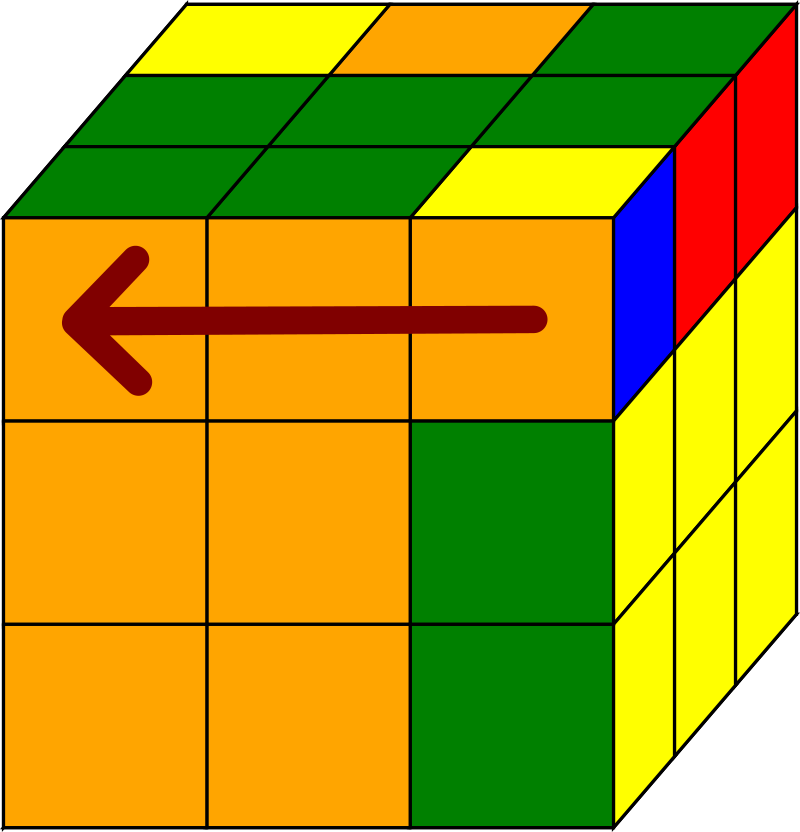
\includegraphics[width=3cm]{images/rubiks-cube.png}
  \end{minipage}
  \begin{minipage}{0.68 \linewidth}
    \begin{haskellcode}
upRows :: RowsLens a
upRows = horizontalSides . liftVec4 topRow

-- Drehe die oberste Ebene im Uhrzeigersinn
moveU :: Aut (RubiksCube a)
moveU =
  cong cube $ cong upRows cycleLeft
            . cong upSide rotateSideCW
    \end{haskellcode}
  \end{minipage}

  \vspace{0.5cm}
  \begin{minipage}{0.7 \linewidth}
    \begin{mdframed}[backgroundcolor=yellow]
      Zur Erinnerung:
      \begin{haskellcode*}{fontsize=\footnotesize}
cong :: Traversal' s a -> Aut a -> Aut s
topRow :: Lens' (Side a) (Vec3 a)
horizontalSides :: Lens' (Cube a) (Vec4 a)
cycleLeft :: Aut (Vec4 a)
rotateSideCW :: Aut (Side a)
      \end{haskellcode*}
    \end{mdframed}
  \end{minipage}
\end{frame}

\begin{frame}[fragile,t]
  \frametitle{Wo kann ich mehr über \haskellinline{lens} erfahren?}
  \begin{itemize}
    \item \textbf{Das Lens-Wiki:} \url{https://github.com/ekmett/lens/wiki}
    \item Blogserie ``Lens over Tea'' \url{http://artyom.me/lens-over-tea-1}
    \item \href{https://skillsmatter.com/skillscasts/4251-lenses-compositional-data-access-and-manipulation}{Vortrag von Simon Peyton Jones bei Skills Matter}
    \item \href{http://www.haskellforall.com/2013/05/program-imperatively-using-haskell.html}{Blogpost: ``Program imperatively using Haskell lenses''}
    \item \href{https://www.fpcomplete.com/school/to-infinity-and-beyond/pick-of-the-week/a-little-lens-starter-tutorial}{School of Haskell: ``A Little Lens Starter Tutorial''}
    \item Cheat Sheet für \verb|Control.Lens|: \\
    \url{https://github.com/anchor/haskell-cheat-sheets}
  \end{itemize}
  \note{Auch ziemlich cool: \href{http://www.haskellforall.com/2015/01/total-100-exhaustive-pattern-matching.html}{total-1.0.0: Exhaustive pattern matching using traversals, prisms, and lenses}}
\end{frame}

{\setbeamertemplate{background}{}
\begin{frame}[b]
  \begin{center}
    
\includegraphics[width=5cm,keepaspectratio]{images/donald-detective.jpg} \\
  \end{center}

  \centering \small
  \url{http://timbaumann.info/lens} \\
  \url{https://github.com/timjb/presentations/tree/gh-pages/lens}
\end{frame}}

\begin{frame}[fragile]
  \frametitle{Plated}
\end{frame}

\begin{frame}[fragile]
  \frametitle{Plated}
  \begin{haskellcode*}{fontsize=\small}
data Inline
  = Str String
  | Emph [Inline]
  | Math MathType String
  | Link [Inline] Target
  | Image [Inline] Target
    ...
  deriving (..., Typeable, Data, Generic)

data Block
  = Para [Inline]
  | BlockQuote [Block]
  | BulletList [[Block]]
  | Header Int Attr [Inline]
    ...
  deriving (..., Typeable, Data, Generic)

data Pandoc = Pandoc Meta [Block]
  deriving (..., Typeable, Data, Generic)
  \end{haskellcode*}
\end{frame}

% TODO:
% Funktionen: over, (&)
% at :: Lens (Map a) (Maybe a)
% Kombinatoren für 'Maybe-Lenses', z.B. (?~)
% Was ist die Konvention mit "Of" am Ende des Namens einer Funktion?
% Lenses für Defaultparameters (https://ocharles.org.uk/blog/posts/2015-07-23-another-approach-to-default-variables.html)

% Bonusfolien:
% * Zippers
% * Plated
% * Indexed Lenses/Traversals
% * Typisomorphismen (da gibts doch so ein Paper...)
% * Semigroups, Apply und Fold1, Traversal1 (siehe Lens over Tea #3)

% Weitere Ideen aus Lens over Tea
% * `Const m` ist ein Applicative wenn m ein Monoid ist. Indem man passende Monide wählt bekommt man view, toListOf, preview, has
% * Typ-Synonyme wie `Getting`, `LensLike`
% * Performance-Probleme bei naiver Implementierung von toListOf
% * `each` bei Traversals
% * `lens-action`

\end{document}
